\documentclass[bachelor, och, labwork]{shiza}

\usepackage[utf8]{inputenc}
\usepackage{graphicx}

\usepackage{pdfpages}

\usepackage[sort,compress]{cite}
\usepackage{amsmath}
\usepackage{amssymb}
\usepackage{amsthm}
\usepackage{fancyvrb}
\usepackage{longtable}
\usepackage{array}
\usepackage[english,russian]{babel}
\usepackage{minted}

\usepackage{tempora}


% \usepackage[colorlinks=false]{hyperref}


\newcommand{\eqdef}{\stackrel {\rm def}{=}}


\begin{document}

\title{}

\course{4}

\group{431}

\napravlenie{10.05.01 "--- Компьютерная безопасность}


\author{Никитина Арсения Владимировича}


\satitle{доцент}
\saname{А.\,В.\,Жаркова}


\date{2022}

\maketitle

% Включение нумерации рисунков, формул и таблиц по разделам
% (по умолчанию - нумерация сквозная)
% (допускается оба вида нумерации)
%\secNumbering


\tableofcontents


\section{Задание лабораторной работы}
Вычислить методом Сильвера-Полига-Хеллмана дискретный логарифм элемента $25$ в 
поле $F_{41}$ отноистельно порождающего элемента $g=7$.


\section{Теоретическая часть}

Пусть $F_q$ --- конечное поле порядка $q=p^r$. Пусть $q-1 = \prod_p{p^{\alpha_p}}$ ---
разложение числа $q-1$ в произведение степеней простых чисел.

Предположим, что все простые делители числа $q-1$ малы. В этом случае примарное 
число $q$ называется гладким. При такой предположениии существует достаточно быстрый
алгоритм нахождения дискретного логарифма в $F_q^*$.

Рассмотрим возможную атаку на дискретный логарифм для гладких $q$.

\begin{center}
    \textit{Алгоритм Сильвера-Полига-Хеллмана}
\end{center}

Пусть $g$ --- порождающий элемент в $F_q^*$.

В начале для каждого простого делителя $p$ числа $q-1$ вычислим все корни $p-$й
степени из 1:

\begin{center}
    $r_{p,j}=g^{j(q-1)/p}, ~j=\overline{0,p-1}$.
\end{center}

Поскольку элемент $g$ является порождающим элементом мультипликативной группы $F_q^*$,
все выписанные элементы различны. Легко проверить, что они являются корнями 
степени $p$ из $1$: $r^p_{p,j} = g^{j(q-1)} = 1, ~j=\overline{0,p-1}$ по Малой
теореме Ферма. В любом поле решений уравнения степени $p$ не более чем $p$, а, 
значит, составленный список полон и больше в нем элементов не прибавится.

Этот шаг проделывается один раз. Его результат --- списки значений $r_{p,j}, ~ j=\overline{0,p-1}$
сохраняются. Обозначим такой список как $\sqrt[p]{1}$.

Рассмотим проблему нахождеия дискретного логарифма:

\begin{center}
    $x:g^x=y$
\end{center}

при различных значениях $y \in F^*_q$.

Заметим, что нам достаточно найти $\forall p ~|~(q-1)$ вычет $x(p)=x(\mathit{mod} ~p^{\alpha_p})$.
Полученные значения $x(p)$ позволяют записать все сравнения $x=x(p)(\mathit{mod}~p^{\alpha_p})$
и вычислить $x$ по Китайской теореме об остатках.

Будем использовать $p-$ичную запись числа $x(p)(\mathit{mod}~p^{\alpha_p})$.

Предположим, что:

\begin{center}
    $x(p) = x_0 + x_1p + x_2p^2 + ... + x_{\alpha_{p}-1}p^{\alpha_p-1} ~(\mathit{mod}~p^{\alpha_p}), ~0 \leqslant x_i < p$.
\end{center}

Для того, чтобы вычислить $x_0$, подсчитаем вначале $y^{(q-1)/p}$. В результате
мы получим корень $p-$й степени из $1$ в $F_q^*$. Так как $y=g^x$, то
$y^{(q-1)/p}=g^{x(q-1)/p}=g^{x_0(q-1)/p}=r_{p,x_0}$.

Сравниваем $r_{p,x_0}$ с элементами $r_{p,j}$, где $0\leqslant j < p$. Находим
такое значение $j$, что $r_{p, x_0}=r_{p,j}$. Значит, $x_0=j$.

Для того, чтобы вычислить $x_1$, заменим $y$ на:

\begin{center}
    $y_1=yg^{-x_0}=g^{x_0+x_1p+...+x_{\alpha - 1}p^{\alpha_p-1 }}$.
\end{center}

Новый элемент $y_1$ имеет дискретный логарифм, равный:

\begin{center}
    $x-x_0=x_1p + ... + x_{\alpha_{p-1}}p^{\alpha_p-1}~(\mathit{mod}~ p^{\alpha_p})$.
\end{center}

Ясно, что $y_1^{(q-1)/p}= 1$. Далее:

\begin{center}
    $y_1^{(q-1)/p^2}=g^{(x-x_0)(q-1)/p^2}=g^{(x_1+x_2p+...)(q-1)/p} = g^{x_1(q-1)/p} = r_{p,x_1}$.
\end{center}

Сравниваем $r_{p,x_1}$ с элементами $\{r_{p,j}\}$. Находим $j:r_{p,x_1}=r_{p,j}$.
Полагаем, $x_1=j$. Продолжаем этот процесс, находим значение:


$$x=x(p)=x_0+x_1p+...+x_{\alpha_{p-1}}p^{\alpha_{p-1}}~(\mathit(mod)~p^{\alpha_p})$$

Далее записываем систему сравнений:

$$x \equiv x_p ~(\mathit{mod} ~p^{\alpha_p})$$

для всех простых делителей $p$ числа $q-1$ и находим $x$, используя Китайсткую
теорему об остатках


\section{Практическая часть}

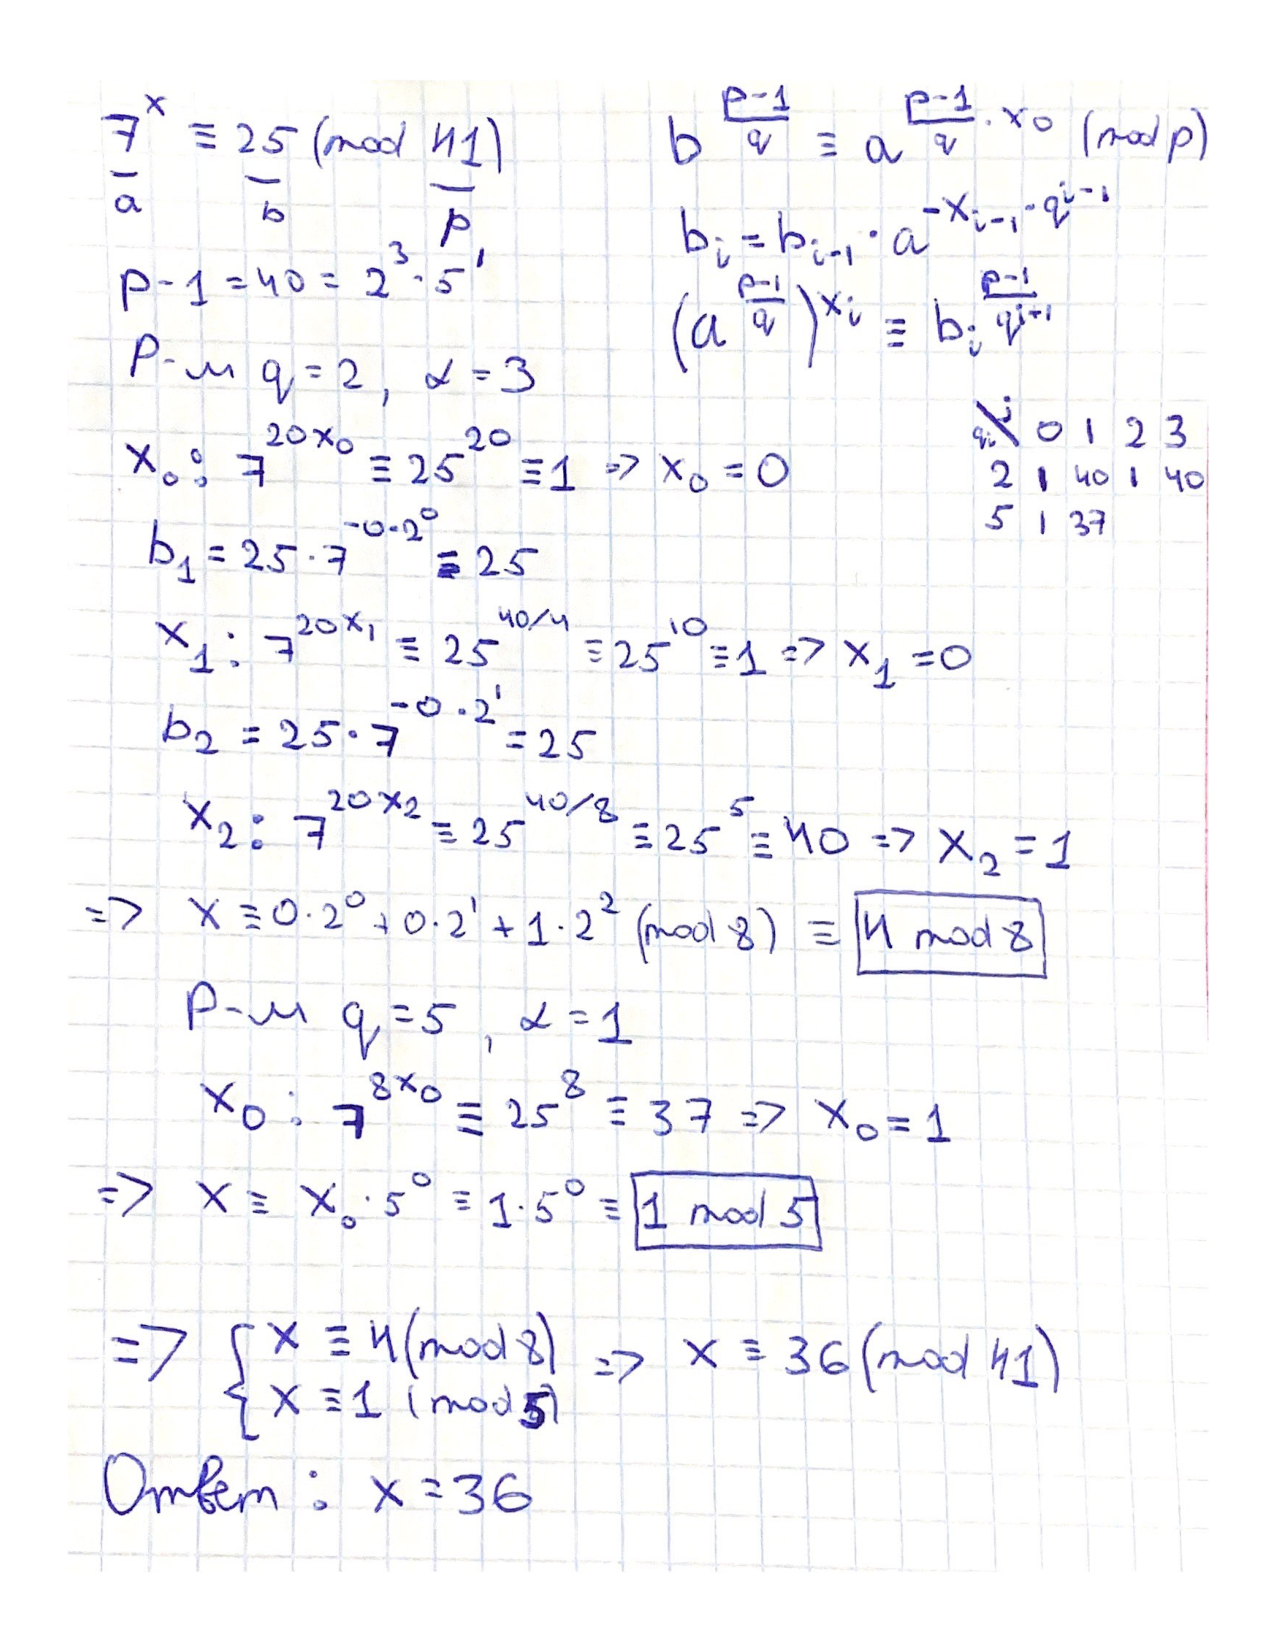
\includepdf[pages={1}, pagecommand=\subsection{Решение задачи}]{2.pdf}\nopagebreak

\subsection{Пример работы алгоритма}
\begin{figure}[H]
    \centering
    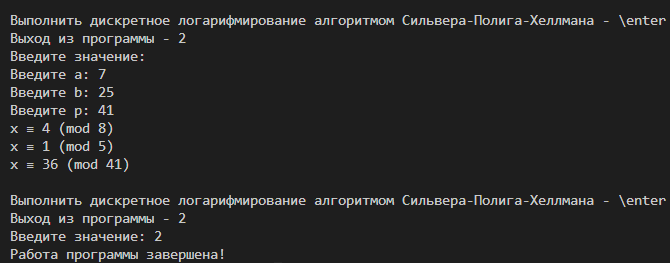
\includegraphics[width=0.8\textwidth]{pic.png}
    \caption{}
\end{figure}


\setminted[python]{linenos,breaklines=true, fontsize=\small, style=bw}
    \subsection{Код программы, реализующей рассмотренный алгоритм}
        \inputminted{python}{lab2.py}

\end{document}